% Chapter 5

\chapter{Result and Discussion}% Main chapter title

\label{Chapter5} % For referencing the chapter elsewhere, use \ref{Chapter} 

\lhead{Chapter 5. \emph{ Result and Discussion }} % This is for the header on each page - perhaps a shortened title

%--------------------------------------------------------------------------------
The dataset we used is originally from BraTS(Brain Tumor Segmentation) dataset.It consists of 

\begin{itemize}
    \item HGG: This folder contains brain images of 220 Patients.There is a
       different folder for each patient. There are 5 different MRI images
       for each Patient. The 5 different images are T1, T2, T1C, FLAIR and
       OT(Ground truth of tumor Segmentation). All these image files
       are stored in .mha format.
       \item LGG - This folder contains brain images of 54 Patients.There is a
       different folder for each patient. There are 5 different MRI images
       for each Patient. The 5 different images are T1, T2, T1C, FLAIR and
       OT(Ground truth of tumor Segmentation). All these image files
       are stored in .mha format.
\end{itemize}
The dataset can be downloaded from: \emph{https://braintumorsegmentation.org/}

\section{Performance of different Machine Learning Algorithms}
We have applied different classification techniques on the above mentioned dataset.  We have allotted 70\% of the data for training and 30\% for testing.  The different classification techniques we used are MLP,  Support Vector Machine, K Nearest Neighbour and Random Forest Classifier.  The results of these classifiers are discussed below:

\begin{table}[h!]
    \centering
    \begin{tabular}{|p{2cm}|l|l|}
    \hline
    \textbf{Classifier} & \textbf{Accuracy}  & \textbf{Loss} \\
    \hline
    MLP & 90.05\% & 0.34\% \\
    \hline
    KNN & 88.55\%  & 0.43\% \\
    \hline
    SVM & 90.04\% & 0.39\% \\
    \hline
    Random Forest & 88.05\% & 0.41\% \\
    \hline
    \end{tabular}
    \caption{Accuracy of different Classifiers}
    \label{tab:my_label}
\end{table}
\newpage
\section{Training of CNN Model}

We used BraTS 2018 dataset for training of our CNN Model. We have divided the dataset into two parts: 70\% for training purpose and 30\% for Validation/testing purpose.

\begin{table}[h!]
    \centering
    \begin{tabular}{|p{2cm}|p{2cm}|}
         \hline
         \textbf{Parameters} & \textbf{Range of values} \\
         \hline
         Number of Epochs & 15 \\
         \hline
         Accuracy & 0.9945 \\
         \hline
         Loss & 0.3777 \\
         \hline
         Best Epoch & 8 \\
         \hline
         Elapsed Time & 39s 222ms/step \\
         \hline
    \end{tabular}
    \caption{Training parameters and values of CNN}
    \label{tab:my_label}
\end{table}

In this model, on using Sigmoid activation function in the dense layer, we achieve an accuracy of 100\% which shows that the network might suffering from a case of overfitness and may work inefficiently for a larger dataset. \\ Thus, we have used ReLU activation function for all convolution layers for which we have achieved 99.45\% accuracy which is an acceptable score for this network.


Plots for the training and Validation are shown below:

 \begin{figure}[htbp]
	    \centering
		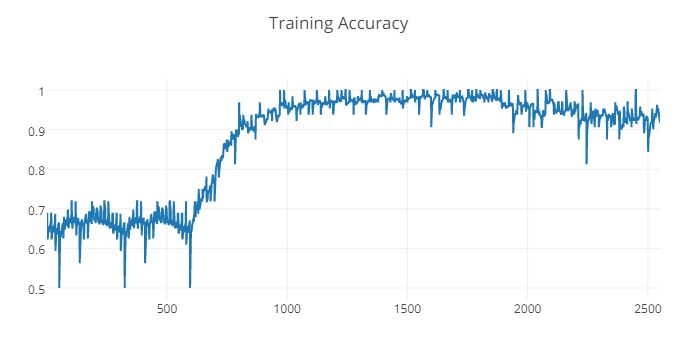
\includegraphics[scale=0.5]{Figures/trainingAccuracy(him).JPG}
		%\rule{10em}{0.5pt}
	    \caption[Training Accuracy]{Training Accuracy}
	    \label{fig:trainccuracy}
        \end{figure}
        
        \begin{figure}[htbp]
	    \centering
		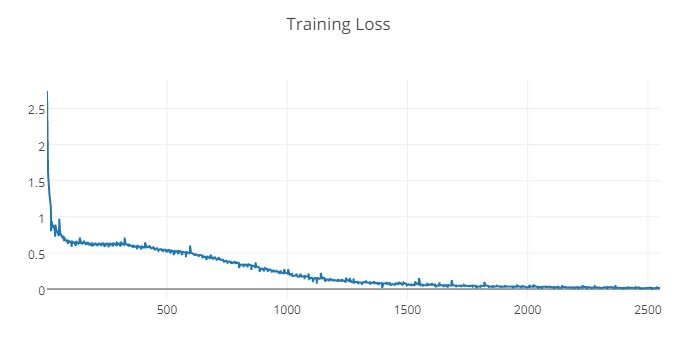
\includegraphics[scale=0.5]{Figures/trainingLoss(him).JPG}
		%\rule{10em}{0.5pt}
	    \caption[Training Loss]{Training Loss}
	    \label{fig:trainloss}
        \end{figure}
        
        
        
        \begin{figure}[htbp]
	    \centering
		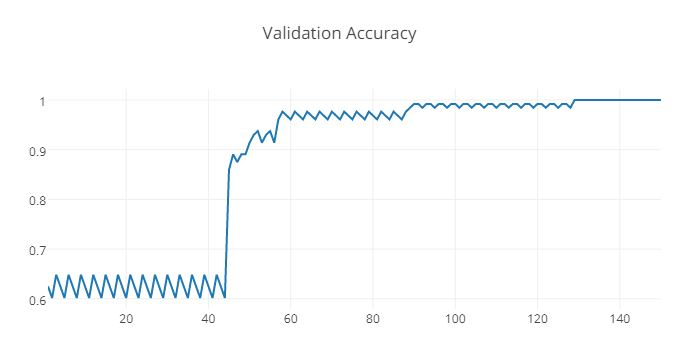
\includegraphics[scale=0.5]{Figures/validationAccuracy(him).JPG}
		%\rule{10em}{0.5pt}
	    \caption[Validation Accuracy]{Validation Accuracy}
	    \label{fig:valacc}
        \end{figure}
        
        \begin{figure}[htbp]
	    \centering
		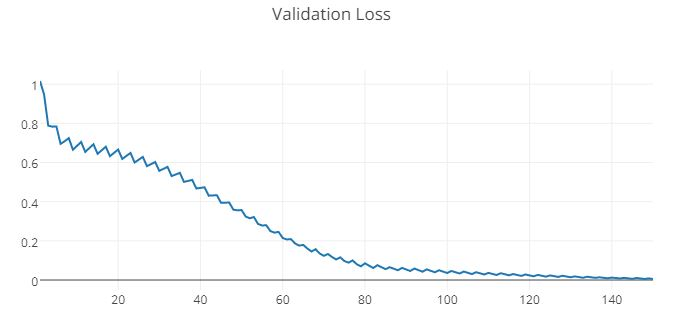
\includegraphics[scale=0.5]{Figures/validationLoss(him).JPG}
		%\rule{10em}{0.5pt}
	    \caption[Validation Loss]{Validation Loss}
	    \label{fig:valloss}
        \end{figure}
        
        \begin{figure}[htbp]
	    \centering
		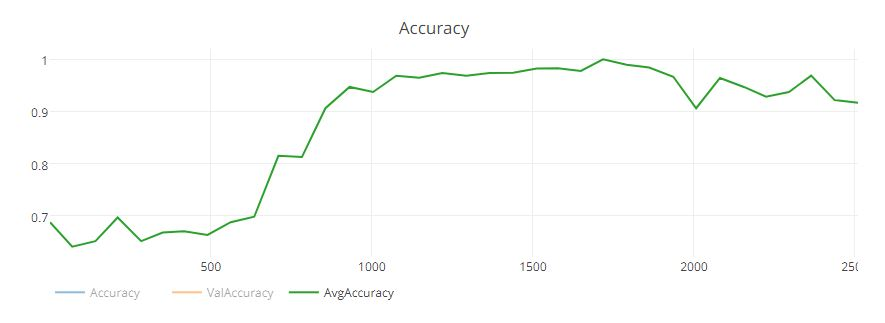
\includegraphics[scale=0.5]{Figures/avgAccuracy(him).JPG}
		%\rule{10em}{0.5pt}
	    \caption[Average Accuracy]{Average Accuracy}
	    \label{fig:avgacc}
        \end{figure}
        
        \begin{figure}[htbp]
	    \centering
		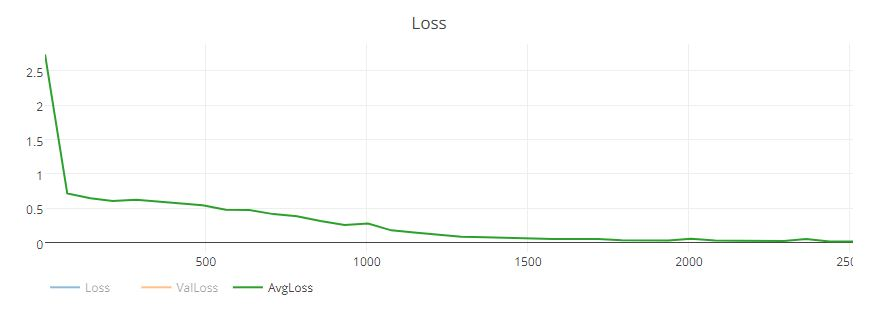
\includegraphics[scale=0.5]{Figures/avgLoss(him).JPG}
		%\rule{10em}{0.5pt}
	    \caption[Average Loss]{Average Loss}
	    \label{fig:avgloss}
        \end{figure}